%                                                                 aa.dem
% AA vers. 9.1, LaTeX class for Astronomy & Astrophysics
% demonstration file
%                                                       (c) EDP Sciences
%-----------------------------------------------------------------------
%
%\documentclass[referee]{aa} % for a referee version
%\documentclass[onecolumn]{aa} % for a paper on 1 column  
%\documentclass[longauth]{aa} % for the long lists of affiliations 
%\documentclass[letter]{aa} % for the letters 
%\documentclass[bibyear]{aa} % if the references are not structured 
%                              according to the author-year natbib style

%
\documentclass{aa}  

%
\usepackage{graphicx}
%%%%%%%%%%%%%%%%%%%%%%%%%%%%%%%%%%%%%%%%
\usepackage{txfonts}
\usepackage{hyperref}
%%%%%%%%%%%%%%%%%%%%%%%%%%%%%%%%%%%%%%%%
%\usepackage[options]{hyperref}
% To add links in your PDF file, use the package "hyperref"
% with options according to your LaTeX or PDFLaTeX drivers.
%
\begin{document} 


   \title{Magnetized Polish doughnuts}

%   \subtitle{}

   \author{Gimeno
          \inst{1}
          \and
          Font\inst{1,2}
          }

   \institute{DAA\\
              \email{wuchterl@amok.ast.univie.ac.at}
         \and
             OAUV \\
             \email{c.ptolemy@hipparch.uheaven.space}
             }

   \date{}

% \abstract{}{}{}{}{} 
% 5 {} token are mandatory
 
  \abstract
  % context heading (optional)
  % {} leave it empty if necessary  
   {}
  % aims heading (mandatory)
   {bla}
  % methods heading (mandatory)
   {bla}
  % results heading (mandatory)
   {bla}
  % conclusions heading (optional), leave it empty if necessary 
   {}

   \keywords{keywords here
               }

   \maketitle
%
%-------------------------------------------------------------------

\section{Introduction}


\citet{Qian:2009} presented a method to build sequences of black hole accretion disks in dynamical equilibria based on
assuming distributions of angular momentum in the disks. Building on this work, we present here the extension of those
models to disks endowed with a purely toroidal magnetic field. For the particular case of constant angular momentum
distributions our method shows good agreement with the results of~\citet{Komissarov:2006}.

In this paper, we consider that the space-time is described by the Kerr metric (test-fluid approximation). We use the geometrized units where $G = c = 1$ and the $(-+++)$ signature for the metric.

%--------------------------------------------------------------------
\section{Framework}

\subsection{Distribution of angular momentum}
First, we introduce the specific angular momentum $l$ and the angular velocity $\Omega$ by the standard definitions,
\begin{equation}
l = - \frac{u_{\phi}}{u_t}, \;\;\; \Omega = \frac{u^{\phi}}{u^t},
\end{equation}
where $u^{\mu}$ is the fluid four-velocity and $g_{\mu\nu}$ is the metric tensor\footnote{In Kerr-Schild coordinates. Although the use of the Boyer-Lindquist coordinates yields exactly the same mathematical derivation and results.}.

The relationship between $l$ and $\Omega$ is given by the equations
\begin{equation}
l = - \frac{\Omega g_{\phi\phi} + g_{t\phi}}{\Omega g_{t\phi} + g_{tt}}, \;\;\; \Omega = - \frac{l g_{tt} + g_{t\phi}}{l g_{t\phi} + g_{\phi\phi}},
\end{equation}
where we are assuming circular motion, i.e. the four-velocity can be written as
\begin{equation}
u^{\mu} = (u^t, 0, 0, u^{\phi}),
\end{equation}
we also introduce the Keplerian angular momentum (for prograde motion) in the equatorial plane $l_{\mathrm{K}}$. 
\begin{equation}\label{eq:kepler}
l_{\mathrm{K}}(r) = \frac{M^{1/2}(r^{2}-2aM^{1/2}r^{1/2}+a^{2})}{r^{3/2}-2Mr^{1/2}+aM^{1/2}},
\end{equation}
In \citet{Jaroszynski:1980} is argued that the slope of the specific angular momentum should be between two cases: $l = \mathrm{const.}$ and $\Omega = \mathrm{const.}$. 

%simulaciones?

We assume the angular momentum distribution proposed by \citet{Qian:2009} 
\begin{equation}
l (r,\theta) = \left\{ \label{eq:ansatz} 
  \begin{array}{lr}
    l_0 \left(\frac{l_{\mathrm{K}}(r)}{l_0}\right)^{\beta}\sin^{2\gamma}{\theta} &  \text{for } r \geq r_{\mathrm{ms}}\\
    l_{\mathrm{ms}}(r)\sin^{2\gamma}{\theta} & \text{for } r < r_{\mathrm{ms}}
  \end{array}
\right\}.
\end{equation}
where $r_{\mathrm{ms}}$ is the radius of the marginally stable circular orbit(INTRODUCIR RMS, RMB Y CUSP ANTES. Introduccion?), the constants $l_0$ and $l_{\mathrm{ms}}(r)$ are defined by $l_0 \equiv \eta l_{\mathrm{K}}(r_{\mathrm{ms}})$ and $l_{\mathrm{ms}}(r) \equiv l_0 [l_{\mathrm{K}}(r_{\mathrm{ms}})/l_0]^{\beta}$. It can be seen that the model for the distribution of angular momentum has three parameters $(\beta, \gamma, \eta)$
\begin{equation}
0 \leq \beta \leq 1, \quad -1 \leq \gamma \leq 1, \quad 1 \leq \eta \leq \eta_{\mathrm{max}},
\end{equation}
with $\eta_{\mathrm{max}} = l_{\mathrm{K}}(r_{\mathrm{mb}})/l_{\mathrm{K}}(r_{\mathrm{ms}})$. In this paper we chose $\eta = \eta_{\mathrm{max}}$, then we can write $l_0$ as $l_0 = l_{\mathrm{K}}(r_{\mathrm{mb}})$. We take this choice because (l comprendido entre lms y lmb para los valores de beta. Discos que comienzan en el cusp no tienen borde exterior para l = lmb.)

\subsection{Magnetized disks}

The equations of ideal GRMHD are
\begin{equation}\label{eq:e-m_cons}
\nabla_{\mu} T^{\mu\nu} = 0,
\end{equation}
\begin{equation}\label{eq:cons_faraday}
\nabla_{\mu} \ast F^{\mu\nu} = 0,
\end{equation}
\begin{equation}\label{eq:continuity}
\nabla_{\mu} (\rho u^{\mu}) = 0,
\end{equation}
where
\begin{equation}\label{eq:e-m_tensor}
T^{\mu\nu} = (w + b^2)u^{\mu}u^{\nu} + \left(p + \frac{1}{2}b^2\right)g^{\mu\nu} - b^{\mu}b^{\nu},
\end{equation}
is the energy-momentum tensor taking into account only the fluid and the Maxwell parts, $w$ and $p$ are the fluid enthalpy and pressure, respectively. And
\begin{equation}
\ast F^{\mu\nu} = b^{\mu}u^{\nu} - b^{\nu}u^{\mu},
\end{equation}
is the Faraday tensor relative to an observer with four-velocity $u^{\mu}$ and $b^{\mu}$ is the magnetic field in that frame.
Assuming the magnetic field is purely azimuthal
\begin{equation}
b^r = b^{\theta} = 0,
\end{equation}
and taking into account that the flow is stationary and axisymmetric, we can see that \eqref{eq:continuity} is always satisfied. The same happens with \eqref{eq:cons_faraday}. Contracting the equation \eqref{eq:e-m_tensor} with the projection tensor $h^{\alpha}_{\beta} = \delta^{\alpha}_{\beta} + u^{\alpha}u_{\beta}$, we arrive at
\begin{equation}
(w + b^2)u_{\nu}\partial_i u^{\nu} + \partial_i\left(p + \frac{b^2}{2}\right) - b_{\nu}\partial_i b^{\nu},
\end{equation}
where the comma denotes partial derivatives and $i = r, \theta$. We can rewrite this equation in terms of the specific angular momentum $l$ and the angular velocity $\Omega$, to obtain

\begin{equation}\label{eq:diff_ver}
\partial_i(\ln u_t|) - \frac{\Omega \partial_i l}{1-l\Omega} + \frac{\partial_i p}{w} + \frac{\partial_i(\mathcal{L}b^2)}{2\mathcal{L}w} = 0,
\end{equation}
where 
\begin{equation}
\mathcal{L} = g_{t\phi}^2 - g_{tt}g_{\phi\phi}.
\end{equation}
To integrate the equation \eqref{eq:diff_ver} first we assume a barotropic equation of state $w = w(p)$ of the form
\begin{equation}\label{eq:eos_fluid}
p = K w^{\kappa},
\end{equation}
with $K$ and $\kappa$ constants.

Then, we define the magnetic pressure as $p_{\mathrm{m}} = b^2/2$. Also, we can define $\tilde{p}_{\mathrm{m}} = \mathcal{L} p_{\mathrm{m}}$ and $\tilde{w} = \mathcal{L} w$, so we can write an analogue of \eqref{eq:eos_fluid} for $\tilde{p}_{\mathrm{m}}$
\begin{equation}\label{eq:eos_mag_tilde}
\tilde{p}_{\mathrm{m}} = K_{\mathrm{m}} \tilde{w}_{\mathrm{m}}^{\eta},
\end{equation}
or, in terms of the magnetic pressure $p_{\mathrm{m}}$
\begin{equation}\label{eq:eos_mag}
p_{\mathrm{m}} = K_{\mathrm{m}} \mathcal{L}^{\eta-1} w^{\eta},
\end{equation}
where $K_{\mathrm{m}}$ and $\eta$ are constants.

This particular choice of relationships $w = w(p)$ and $\tilde{w} = \tilde{w}(\tilde{p}_{\mathrm{m}})$, fulfill the general relativistic version for a toroidal magnetic field of the von Zeipel theorem \citep{vonZeipel1924, Zanotti2015}, that means the surfaces of $\Omega$ and $l$ constant coincide.

We can rewrite equation \eqref{eq:diff_ver} and integrate it to give
\begin{equation}\label{eq:pre_full_int}
\ln |u_t| - \int^l_0 \frac{\Omega \mathrm{d}l}{1 - \Omega l} + \int^p_0 \frac{\mathrm{d}p}{w} + \int^{\tilde{p}_{\mathrm{m}}} \frac{\mathrm{d}\tilde{p}_{\mathrm{m}}}{\tilde{w}} = \mathrm{constant}.
\end{equation}
On the surface of the disk, and particularly on its inner edge,
\begin{equation}
p = \tilde{p}_{\mathrm{m}} = 0, \;\;\; u_t = u_{t, \mathrm{in}}, \;\;\; l = l_{\mathrm{in}}
\end{equation}
then, the constant of integration is given by
\begin{equation}
\mathrm{constant.} = \ln |u_t| - \int^l_{\mathrm{in}} \frac{\Omega \mathrm{d}l}{1 - \Omega l}.
\end{equation}
Defining the total potential $W$ \citet{Abramowicz:1978}, we can write
\begin{equation}\label{eq:potential}
W - W_{\mathrm{in}} = \ln|u_t| - \ln|u_{t,\mathrm{in}}| - \int^{l}_{l_{\mathrm{in}}} \frac{\Omega \mathrm{d}l}{1 - \Omega l},
\end{equation}
where $W_{\mathrm{in}}$ is the potential on the inner edge of the disk. With this definition, we can write \eqref{eq:pre_full_int} as
\begin{equation}\label{eq:full_int}
W - W_{\mathrm{in}} = \int^p_0 \frac{\mathrm{d}p}{w} + \int^{\tilde{p}_{\mathrm{m}}} \frac{\mathrm{d}\tilde{p}_{\mathrm{m}}}{\tilde{w}},
\end{equation}
and
\begin{equation}\label{eq:pre_enthalpy_eq}
W - W_{\rm{in}} + \frac{\kappa}{\kappa - 1}\frac{p}{w} + \frac{\eta}{\eta - 1}\frac{p_{\mathrm{m}}}{w} = 0,
\end{equation}
and then, replacing $p$ and $p_{\mathrm{m}}$ by equations \eqref{eq:eos_fluid} and \eqref{eq:eos_mag},
\begin{equation}\label{eq:enthalpy_eq}
W - W_{\rm{in}} + \frac{\kappa}{\kappa - 1} K w^{\kappa - 1} + \frac{\eta}{\eta - 1}K_{\mathrm{m}}(\mathcal{L} w)^{\eta - 1} = 0,
\end{equation}
which relates the distribution of potential with the distribution of enthalpy.

%--------------------------------------------------------------------
\section{Methodology}

\subsection{Building the disk}

To construct the disks we follow the procedure described below:

First, we find the location of $r_{\mathrm{cusp}}$ and $r_{\mathrm{c}}$ as the solutions to the equation $l(r) - l_{\mathrm{K}} = 0$.
Next, we write the partial derivatives of the potential \eqref{eq:potential}
\begin{equation}\label{eq:radial_der_pot}
\partial_r W = \partial_r \ln|u_t| - \frac{\Omega \partial_rl}{1 - \Omega l},
\end{equation}
and
\begin{equation}\label{eq:polar_der_pot}
\partial_{\theta} W = \partial_{\theta} \ln|u_t| - \frac{\Omega \partial_{\theta}l}{1 - \Omega l}.
\end{equation}
Then, we integrate the radial partial derivative of the potential along the segment $[r_{\mathrm{cusp}}, r_{\mathrm{c}}]$ (assuming $W_{\mathrm{cusp}} = 0$) at the equatorial plane, thus obtaining the equatorial distribution of potential between $r_{\mathrm{cusp}}$ and $r_{\mathrm{c}}$
\begin{equation}\label{eq:equatorial_pot}
W_{\mathrm{eq}}(r) = \int^{r}_{r_{\mathrm{cusp}}}\left(\partial_r \ln|u_t| - \frac{\Omega \partial_rl}{1 - \Omega l}\right).
\end{equation}
We can divide the equations \eqref{eq:radial_der_pot} and \eqref{eq:polar_der_pot} \citep{Qian:2009} to get
\begin{equation}\label{eq:F}
F(r, \theta) = -\frac{\partial_r W}{\partial_{\theta} W} = \frac{\mathrm{d}\theta}{\mathrm{d}r}.
\end{equation}
which is an ordinary differential equation that can be integrated to obtain the location of the equipotential surfaces.

Next, we choose all the initial values for the integration of the equation \eqref{eq:F} to be between $r_{\mathrm{cusp}}$ and $r_{\mathrm{c}}$ ($\theta = \pi / 2$). Since we are only interested in the surfaces inside the Roche lobe, our choice of initial values provides us a mapping of the equipotential surfaces of the torus. Given that we have already obtained both the equipotential surfaces which cross the segment $[r_{\mathrm{cusp}}, r_{\mathrm{c}}]$ and the potential distribution there, we found the potential distribution for the torus.
Once we have the potential distribution, we can find the gas pressure at the center, from equation \eqref{eq:enthalpy_eq}
\begin{equation}
p_{\mathrm{c}} = w_{\mathrm{c}}(W_{\mathrm{in}} - W_{\mathrm{c}})\left(\frac{\kappa}{\kappa - 1} + \frac{\eta}{\eta - 1}\frac{1}{\beta_c}\right)^{-1},
\end{equation}

\subsection{Numerical code}

- Description of the numerical construction. 

\subsection{Parameter space}

Parameters $\beta$, $\gamma$, $\eta$, $\beta_{\rm{mag}}$, $\kappa$, $\eta$, $r_{\rm{in}}$ and $a$. We do not vary $\kappa$ and $\eta$. And take $\eta = \eta_{max}$ for each value of $a$

%--------------------------------------------------------------------
\section{Results}

\begin{figure*}
\centering
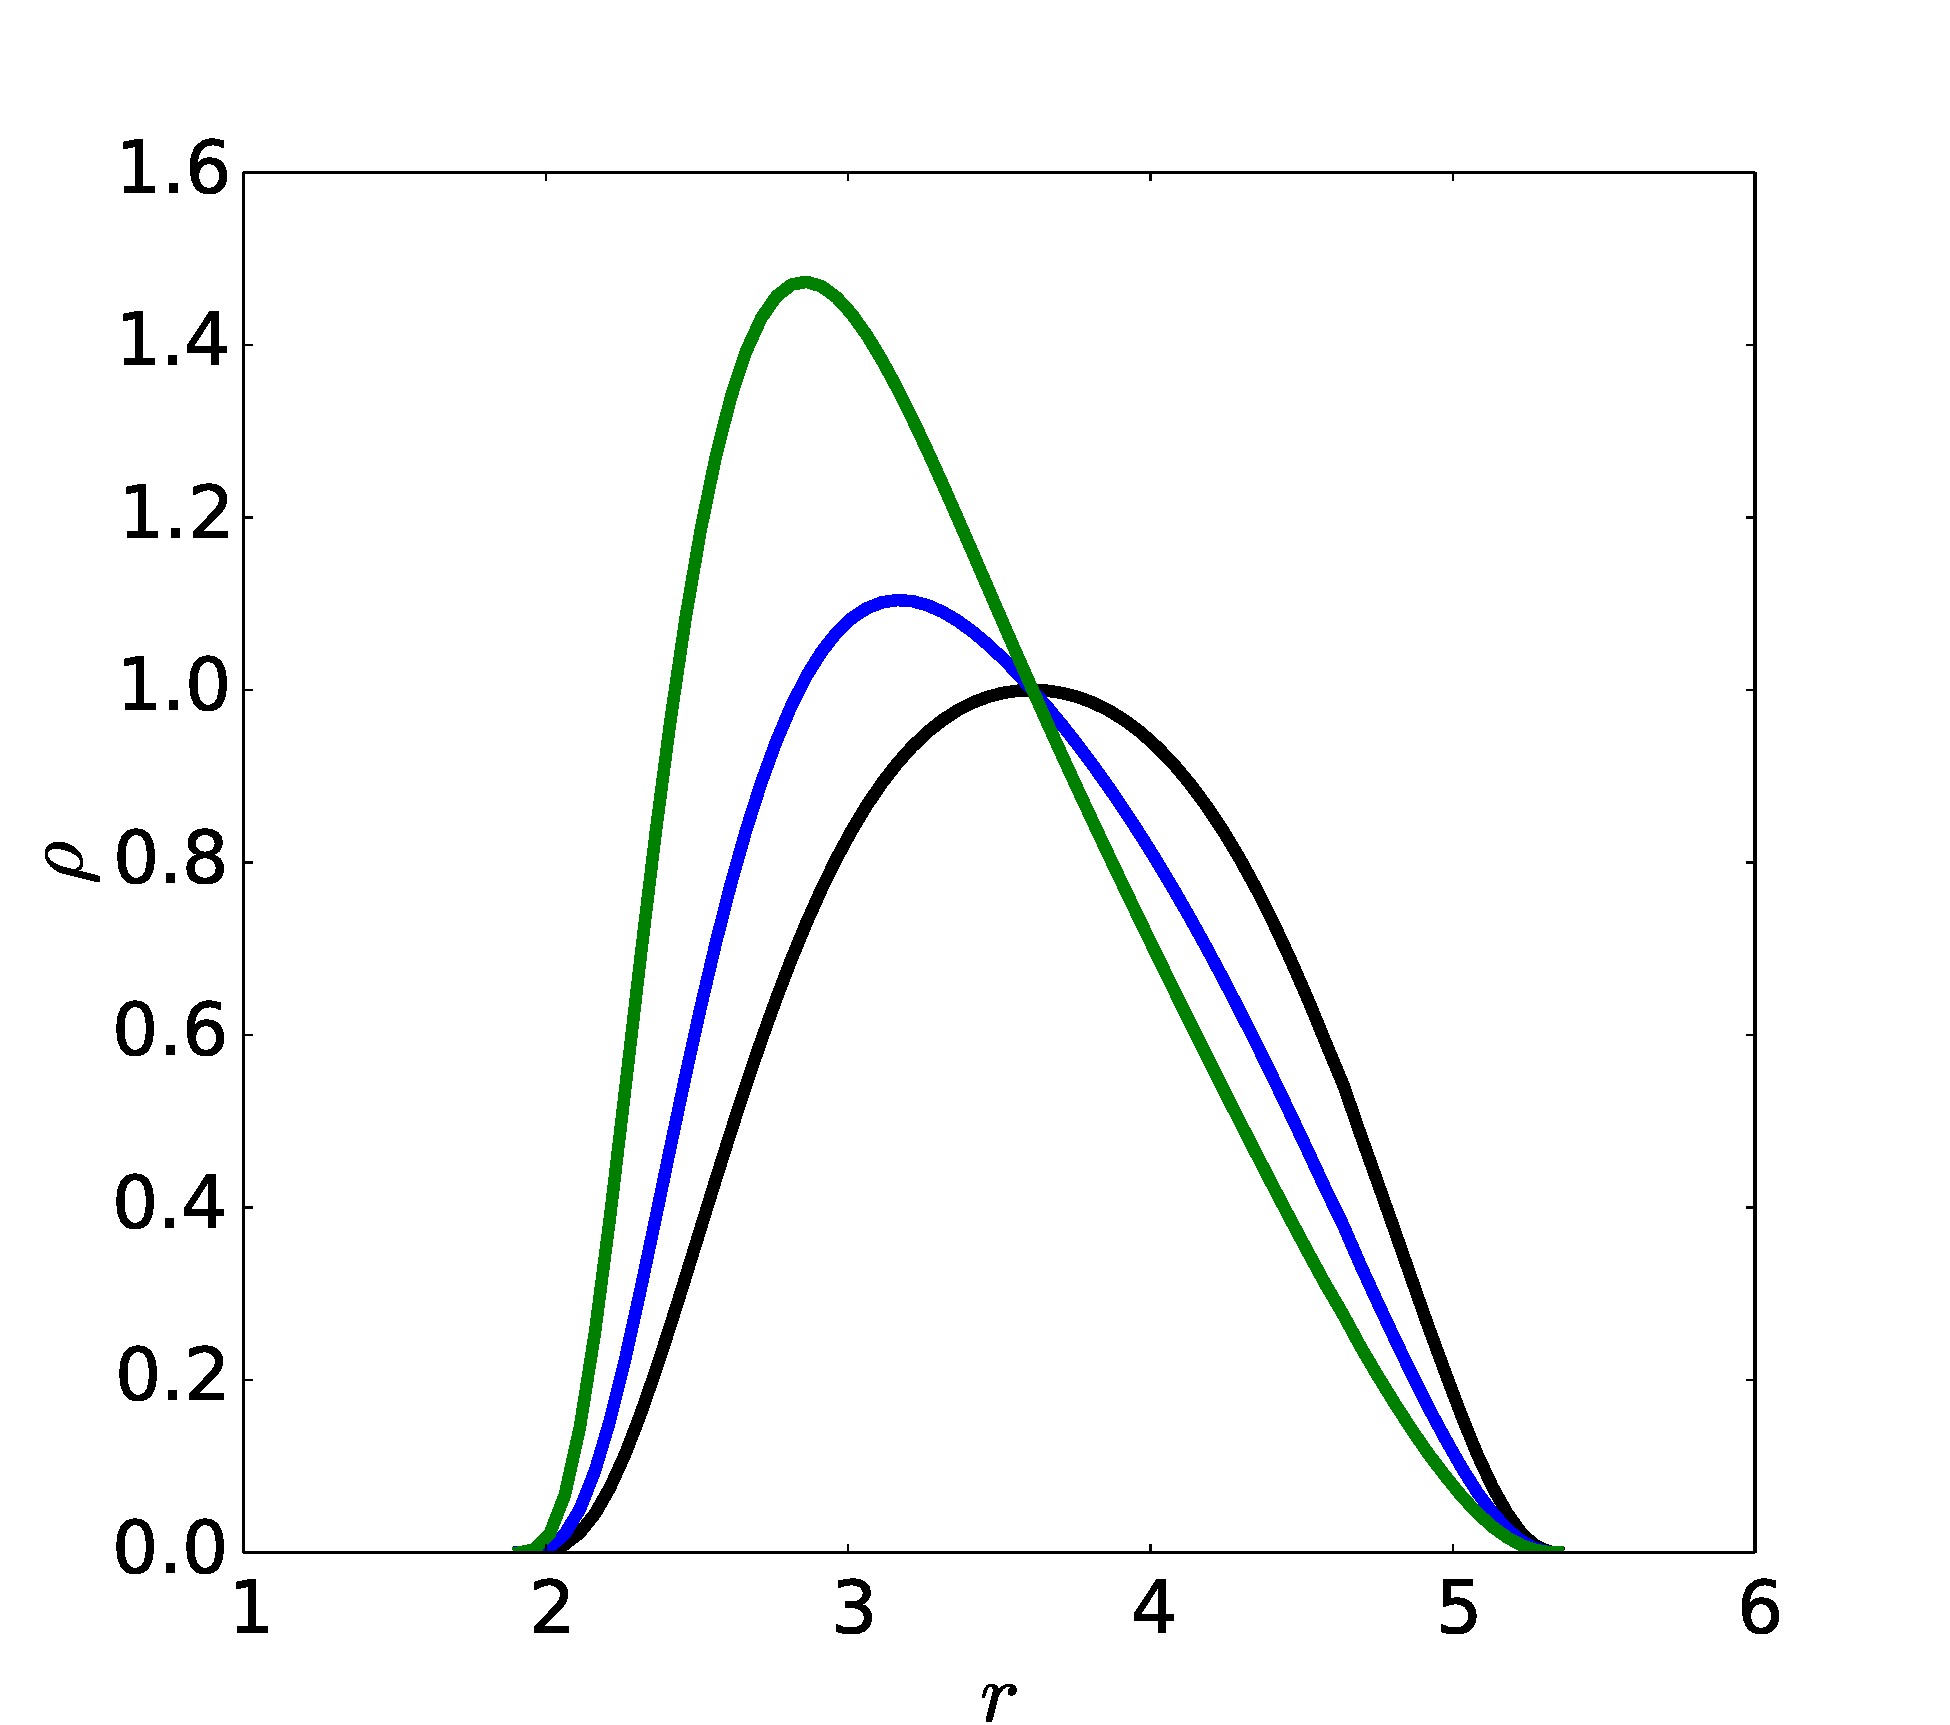
\includegraphics[scale=0.4]{1.pdf}
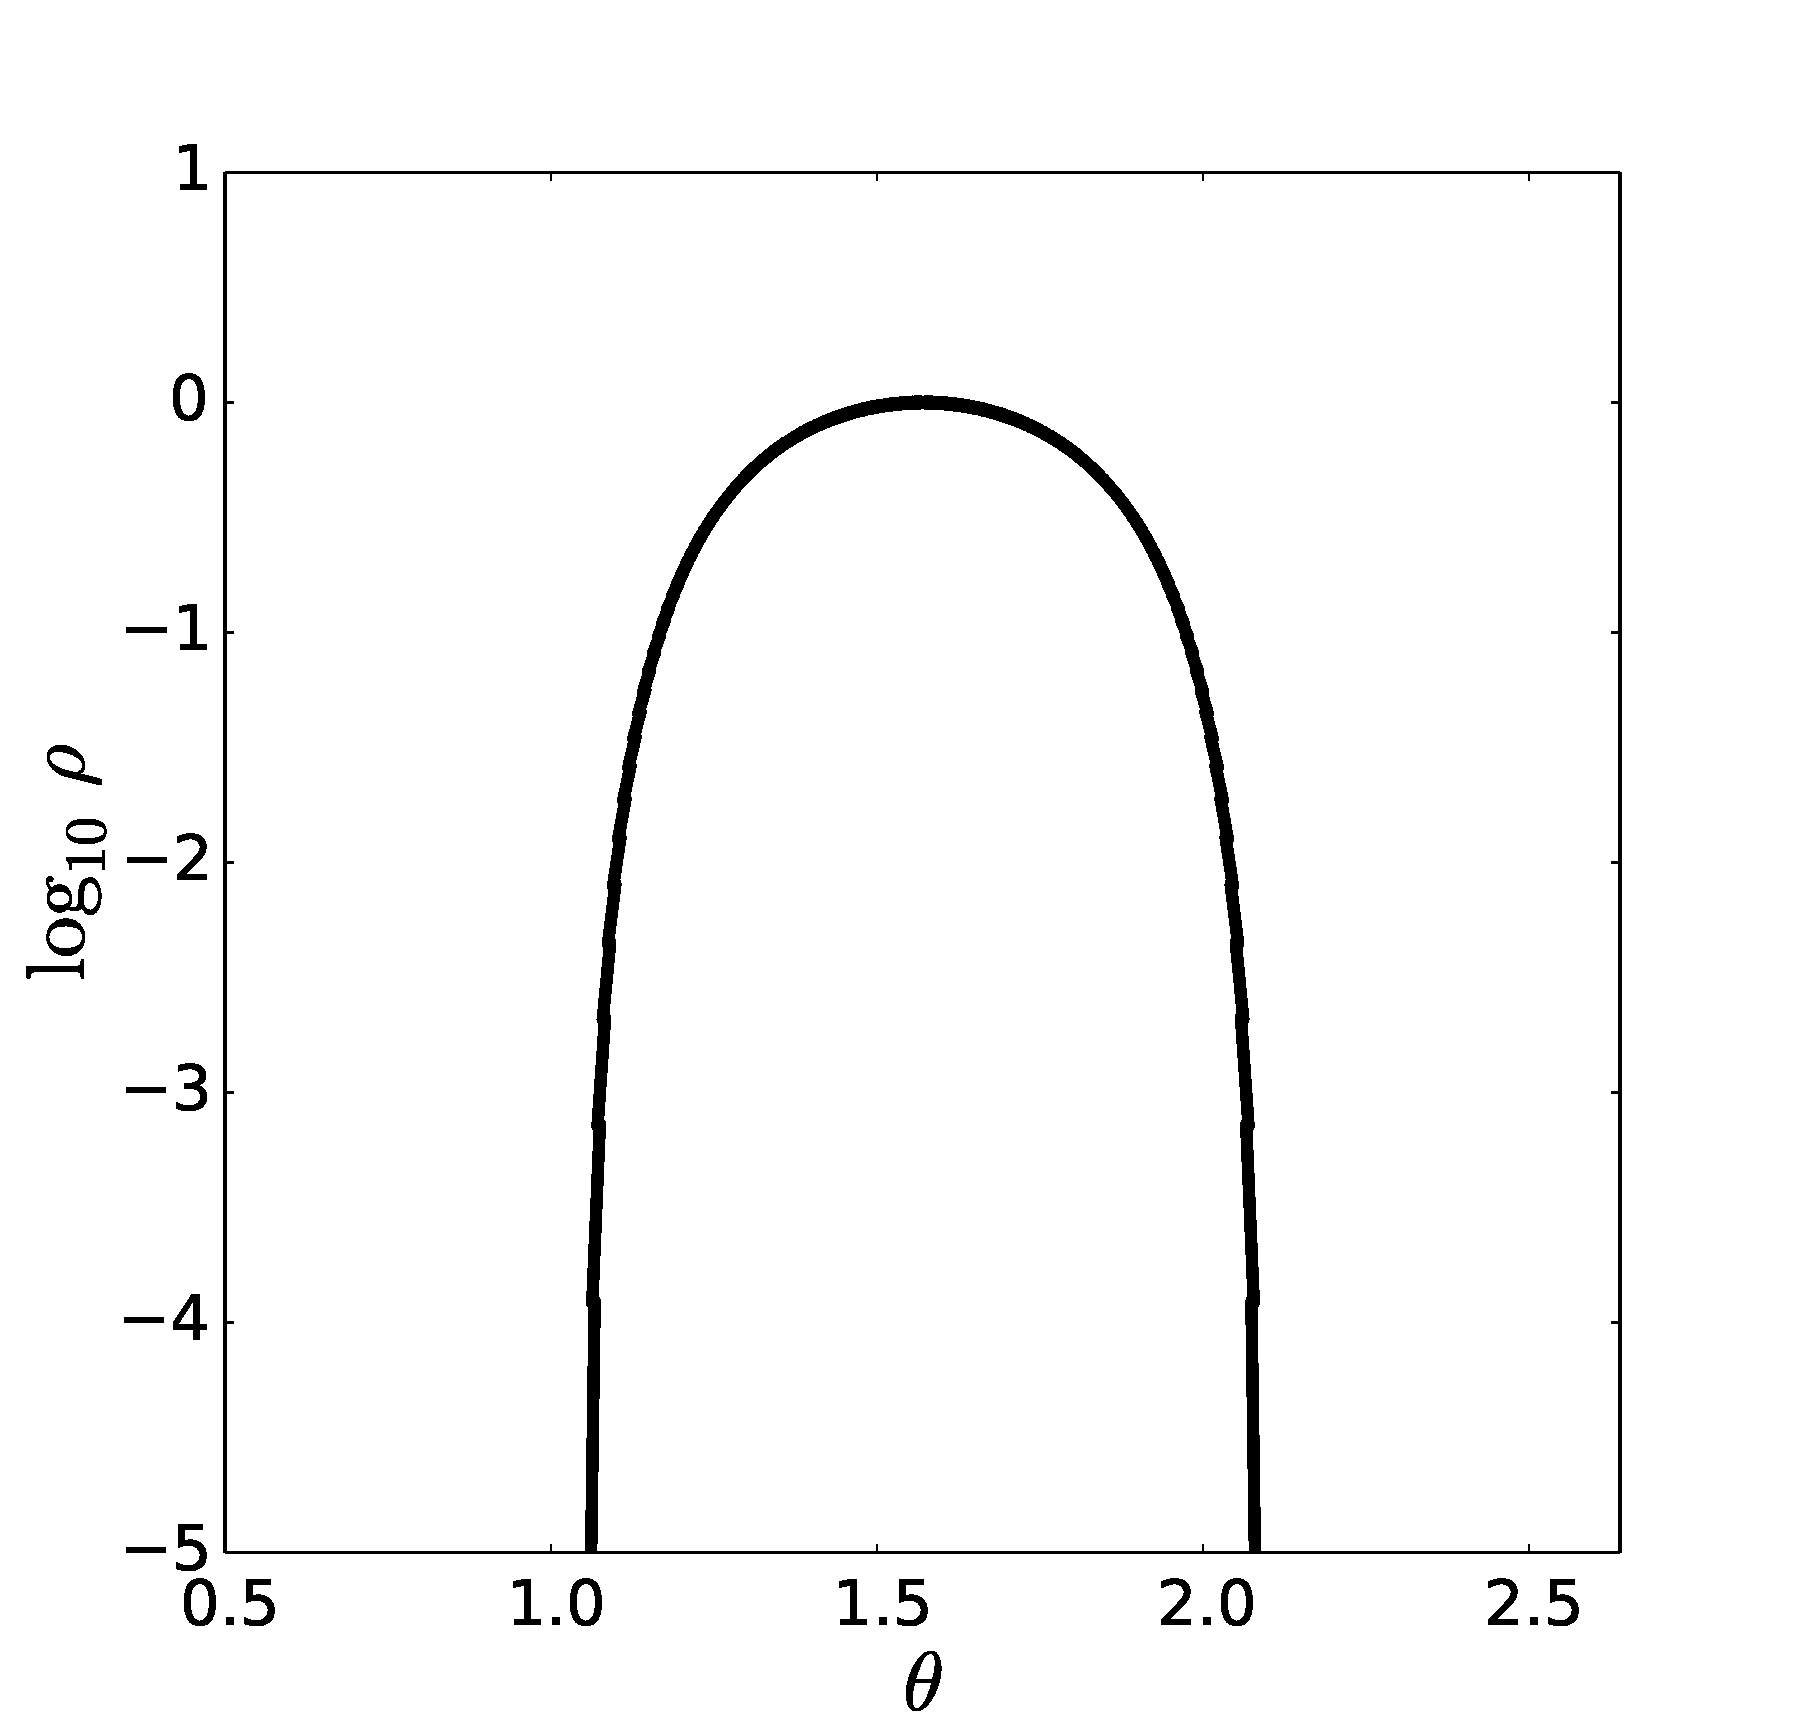
\includegraphics[scale=0.4]{2.pdf}
\caption{Adiabatic exponent $\Gamma_1$.
            $\Gamma_1$ is plotted as a function of
            $\lg$ internal energy $\mathrm{[erg\,g^{-1}]}$ and $\lg$
            density $\mathrm{[g\,cm^{-3}]}$.}
           \label{FigGam}%
 \end{figure*}


%--------------------------------------------------------------------
\section{Conclusions}

%-------------------------------------- Two column figure (place early!)
%   \begin{figure*}
%   \centering
%   %%%\includegraphics{empty.eps}
%   %%%\includegraphics{empty.eps}
%   %%%\includegraphics{empty.eps}
%   \caption{Adiabatic exponent $\Gamma_1$.
%               $\Gamma_1$ is plotted as a function of
%               $\lg$ internal energy $\mathrm{[erg\,g^{-1}]}$ and $\lg$
%               density $\mathrm{[g\,cm^{-3}]}$.}
%              \label{FigGam}%
%    \end{figure*}
%


%--------------------------------------------------- One column table
%   \begin{table}
%      \caption[]{Opacity sources.}
%         \label{KapSou}
%     $$ 
%         \begin{array}{p{0.5\linewidth}l}
%            \hline
%            \noalign{\smallskip}
%            Source      &  T / {[\mathrm{K}]} \\
%            \noalign{\smallskip}
%            \hline
%            \noalign{\smallskip}
%            Yorke 1979, Yorke 1980a & \leq 1700^{\mathrm{a}}     \\
%%           Yorke 1979, Yorke 1980a & \leq 1700             \\
%            Kr\"ugel 1971           & 1700 \leq T \leq 5000 \\
%            Cox \& Stewart 1969     & 5000 \leq             \\
%            \noalign{\smallskip}
%            \hline
%         \end{array}
%     $$ 
%   \end{table}
%



\begin{acknowledgements}
      Bla, bla, bla.
\end{acknowledgements}

% WARNING
%-------------------------------------------------------------------
% Please note that we have included the references to the file aa.dem in
% order to compile it, but we ask you to:
%
% - use BibTeX with the regular commands:
%   \bibliographystyle{aa} % style aa.bst
%   \bibliography{references.bib} % your references Yourfile.bib
%
% - join the .bib files when you upload your source files
%-------------------------------------------------------------------

\bibliographystyle{bibtex/aa}
\bibliography{references}

\end{document}
